\section{Experimental Results}
\label{sec:experimental_results}
The proposed architecture is demonstrated on a Xilinx Zynq-7020. This device integrates a dual ARM Cortex-A9 based \gls{ps} and \gls{pl} equivalent to Xilinx Artix-7 (\gls{fpga}) in a single chip \cite{xilinx2015zynq}. The Zynq-7020 architecture conveniently maps the custom logic and software in the \gls{pl} and \gls{ps} respectively as an embedded system.

In this platform, the proposed hardware architecture is implemented to deploy the \gls{sbs} network structure shown in \ref{fig:sbs_network} for handwritten digit classification task for MNIST data set. The \gls{sbs} model is trained using standard floating-point. Matlab software is used for this \gls{sbs} network implementation. The resulting synaptic weight matrices are deployed on the embedded system as binary files stored in a micro SD memory card. In the embedded software, the \gls{sbs} network is built as a sequential model using the \gls{api} from the \gls{sbs} embedded software framework \cite{nevarez2020accelerator}. This \gls{api} allows to configure the computational workload of the neural network, this can be distributed among the hardware processing units and the embedded \gls{cpu}.

For the evaluation of this approach, it is presented a design exploration by reviewing the computational latency, inference accuracy, resource utilization, and power dissipation. First, the performance of the embedded \gls{cpu} is taken as benchmark, and then repeat the measurements on hardware processing units with standard floating-point computation. Afterwards, the dot-product architecture is evaluated addressing a design exploration with hybrid custom floating-point approximation, as well as the hybrid logarithmic approximation. Finally, a discussion of results is presented.


\subsection{Performance Benchmark}
\subsubsection{Benchmark on Embedded CPU}

The performance of the \gls{cpu} for \gls{sbs} network inference is examined. In this case, the embedded software builds the \gls{sbs} network as a sequential model mapping the entire computation to the \gls{cpu} (ARM Cortex-A9) at \unit[666]{MHz} and a power dissipation of \unit[1.658]{W}.

The \gls{sbs} network computation on the \gls{cpu} reaches a latency of \unit[34.28]{ms} per spike with accuracy of \unit[99.3]{\%} correct classification on the $10,000$ image test set with $1000$ spikes. The latency and schedule of the \gls{sbs} network computation are displayed in \Tab{tab:latency_sw} and \Fig{fig:latency_sw}, respectively.

\begin{table}[!t]\centering
	\caption{Computation on embedded CPU.}\label{tab:latency_sw}
	\scriptsize
\begin{tabular}{lrr}\toprule
	\textbf{Layer} &\textbf{Latency (ms)} \\\midrule
	HX\_IN &1.184 \\
	H1\_CONV &4.865 \\
	H2\_POOL &3.656 \\
	H3\_CONV &20.643 \\
	H4\_POOL &0.828 \\
	H5\_FC &3.099 \\
	HY\_OUT &0.004 \\
		
	TOTAL &34.279 \\
	\bottomrule
\end{tabular}
\end{table}

\begin{figure*}[b!]
	\centering
	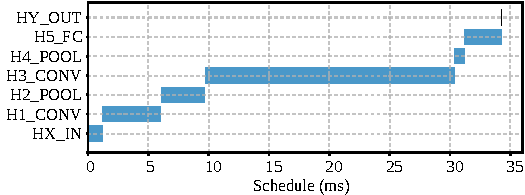
\includegraphics[width=0.5\columnwidth]{./chapters/sbs_accelerator/figures/latency_sw.pdf}
	\caption{Computation on embedded CPU.}
	\label{fig:latency_sw}
\end{figure*}

\subsubsection{Benchmark on Processing Units with Standard Floating-Point Computation}
The system architecture shown in \Fig{fig:hw_sbs_8_pu} is implemented to benchmark the computation on hardware \glspl{pu} with standard floating-point. The embedded software builds the \gls{sbs} network as a sequential model and delegates the network computation to the hardware processing units at \unit[200]{MHz} as clock frequency.

\begin{figure*}[b!]
	\centering
	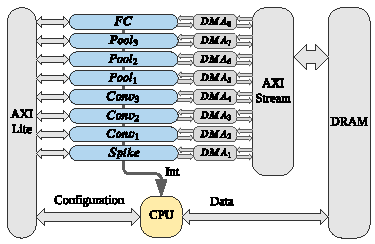
\includegraphics[width=0.5\columnwidth]{./chapters/sbs_accelerator/figures/sbs_hw_experimental.pdf}
	\caption{System overview of the top-level architecture with 8 processing units.}
	\label{fig:hw_sbs_8_pu}
\end{figure*}

The layers of the neural network with the most neurons are partitioned for asynchronous parallel processing. Since \emph{H2\_POOL} and \emph{H3\_CONV} are the layers with the most neurons, the computational workload is distributed between two \glspl{pu} for each one of these layers. The output layer \emph{HY\_OUT} is fully processed by the \gls{cpu}, since it is the layer with fewest neurons. The hardware mapping and the computation schedule of this deployment are displayed in \Tab{tab:latency_fp} and \Fig{fig:latency_pu_fp}, respectively.

\begin{table}[!t]\centering
	\caption{Performance of processing units with standard floating-point (IEEE 754) computation.}\label{tab:latency_fp}
	\scriptsize
	\begin{tabular}{llrrrrrr}\toprule
		\multicolumn{2}{c}{\textbf{Hardware mapping}} & &\multicolumn{4}{c}{\textbf{Computation schedule (ms)}} \\\cmidrule{1-2}\cmidrule{4-7}
		\textbf{Layer} &\textbf{PU} & &$t_s$ &$t_{CPU}$ &$t_{PU}$ &$t_f$ \\\midrule
		HX\_IN &Spike & &0 &0.056 &0.370 &0.426 \\
		H1\_CONV &Conv1 & &0.058 &0.598 &2.002 &2.658 \\
		\multirow{2}{*}{H2\_POOL}
		&Pool1 & &0.658 &0.126 &1.091 &1.875 \\
		&Pool2 & &0.785 &0.125 &1.075 &1.985 \\
		\multirow{2}{*}{H3\_CONV} 
		&Conv2 & &0.911 &0.280 &3.183 &4.374 \\
		&Conv3 & &1.193 &0.279 &3.176 &4.648 \\
		H4\_POOL &Pool3 & &1.473 &0.037 &0.481 &1.991 \\
		H5\_FC &FC & &1.512 &0.101 &1.118 &2.731 \\
		HY\_OUT &CPU & &1.615 &0.004 &0 &1.619 \\
		\bottomrule
	\end{tabular}
\end{table}

\begin{figure*}[b!]
	\centering
	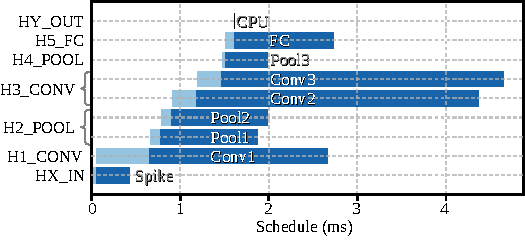
\includegraphics[width=0.5\columnwidth]{./chapters/sbs_accelerator/figures/latency_pu_fp.pdf}
	\caption{Performance of processing units with standard floating-point (IEEE 754) computation.}
	\label{fig:latency_pu_fp}
\end{figure*}

In the computation schedule, the following terms are defined as follows: $t_s(n)$ as the start time for the processing of the neural network layer (as a compute node) $n\in L$ where $L$ represents the set of layers; $t_{CPU}(n)$ as the \gls{cpu} preprocessing time; $t_{PU}(n)$ as the \gls{pu} latency; and $t_f(n)$ as the finish time. For data preparation, $t_{CPU}(n)$ is the duration in which the \gls{cpu} writes a DRAM buffer with $\vec{h}_\mu$ (vector of neuron latent variables) of the current processing layer and $S_t$ (input spike matrix) from its preceding layer. This buffer is streamed to the \gls{pu} via \gls{dma}.

The total execution time of the \gls{cpu} is defined by \Equ{eq:time_cpu}. In a cyclic spiking inference, the execution time of the network computation is the longest path among the processing units including the \gls{cpu}. This is denoted as the latency of an spike cycle and it is defined by \Equ{eq:time_spike}. The total execution time of the network computation is the last finish time ($t_f$) in the schedule defined by \Equ{eq:time_finish}.

\begin{figure*}[b!]
	\centering
	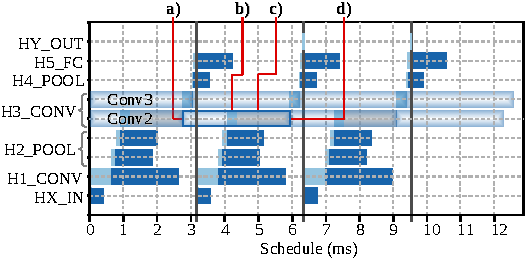
\includegraphics[width=0.5\columnwidth]{./chapters/sbs_accelerator/figures/latency_fp_cycle.pdf}
	\caption{Performance bottleneck of cyclic computation on processing units with standard floating-point (IEEE 754) arithmetic, (a) exhibits the starting of $t_{PU}$ of \emph{Conv2} on a previous computation cycle, (b) presents $t_{CPU}$ of \emph{Conv2} on the current computation cycle, (c) shows the CPU waiting time (in gray color) for \emph{Conv2} as a busy resource (awaiting for \emph{Conv2} interruption), and (d) illustrates the $t_{f}$ from the previous computation cycle, the starting of $t_{PU}$ on the current computation cycle (\emph{Conv2} interruption on completion, and start current computation cycle).}
	\label{fig:latency_pu_fp_cycle}
\end{figure*}

\begin{eqnarray} \label{eq:time_cpu}
T_{CPU} = \sum_{n\in L} t_{CPU}(n)
\end{eqnarray}

\begin{eqnarray} \label{eq:time_pu}
T_{PU} = \max_{n\in L}(t_{PU}(n))
\end{eqnarray}

\begin{eqnarray} \label{eq:time_spike}
T_{SC} =
\begin{cases}
T_{PU}, & \text{if}\ T_{CPU}\le T_{PU} \\
T_{CPU}, & \text{otherwise}
\end{cases}
\end{eqnarray}

\begin{eqnarray} \label{eq:time_finish}
T_{f} = \max_{n\in L}(t_{f}(n))
\end{eqnarray}

Using standard floating-point requires a high computational cost. As the largest layer, the computational workload of \emph{H3\_CONV} is evenly partitioned among two \glspl{pu}: \emph{Conv2} and \emph{Conv3}. However, in the cyclic schedule, \emph{Conv2} causes the performance bottleneck as shown in \Fig{fig:latency_pu_fp_cycle}. In this case, the \gls{cpu} awaits for \emph{Conv2} to finish the computation of the previous cycle in order to start the current computation cycle. In contrast, as the smallest layer, the computational workload of \emph{HY\_OUT} is fully processed by the \gls{cpu}. \Tab{tab:latency_fp} and \Fig{fig:latency_pu_fp} show \unit[4]{$\mu$s} as the processing latency of \emph{HY\_OUT}. This latency is negligible compared to the overall performance assessment. Accelerating \emph{HY\_OUT} would yield a negligible gain. Moreover, assigning a dedicated hardware \gls{pu} to \emph{HY\_OUT} would add unprofitable data transfer and hardware interruption handling overheads.

Applying \Equ{eq:time_spike}, it is obtained a latency of \unit[3.18]{ms} per spike cycle. This deployment achieves an accuracy of $98.98\%$ correct classification on the $10,000$ image test set with $1000$ spikes.

The post-implementation resource utilization and power dissipation are shown in \Tab{tab:resource_fp}. Each \emph{Conv} \gls{pu} instantiates an on-chip stationary weight matrix of $52,000$ entries, wish is sufficient to store $W\in\mathbb{R}^{5\times 5\times 2\times 32}$ and $W\in\mathbb{R}^{5\times 5\times 32\times 64}$ for \emph{H1\_CONV} and \emph{H3\_CONV}, respectively. In order to reduce BRAM utilization, a custom floating-point representation is used, composed of a 4-bit exponent and a 4-bit mantissa (bit sign is omitted). Each 8-bit entry is promoted to its standard floating-point representation for the dot-product computation. The method to find the appropriate bit-width parameters for custom floating-point representation is presented in Section~\ref{sec:parameters}.

\begin{table}[!h]\centering
	\caption{Resource utilization and power dissipation of processing units with standard floating-point (IEEE 754) computation.}\label{tab:resource_fp}
	\scriptsize
	\begin{tabular}{lrrrrrrr}\toprule
		\textbf{PU} & &\textbf{LUT} &\textbf{FF} &\textbf{DSP} &\textbf{BRAM 18K} &\textbf{Power (mW)} \\\midrule
		Spike & &2,640 &4,903 &2 &2 &38 \\
		Conv & &2,765 &4,366 &19 &37 &89 \\
		Pool & &2,273 &3,762 &5 &3 &59 \\
		FC & &2,649 &4,189 &8 &9 &66 \\
		\bottomrule
	\end{tabular}
\end{table}

%\begin{figure}[!h]
%	\centering
%	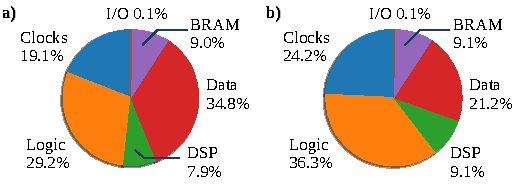
\includegraphics[width=1\columnwidth]{../figures/power_dissipation_breakdown_float-32.pdf}
%	\caption{Power dissipation breakdown of processing units with standard floating-point (IEEE 754), (a) \emph{Conv}, and (b) \emph{FC}.}
%	\label{fig:power_dissipation_breakdown_float_32}
%\end{figure}

The implementation of dot-product with standard floating-point arithmetic (IEEE 754) utilizes proprietary Xilinx multiplier and adder floating-point operator cores. Vivado \gls{hls} implements floating-point arithmetic operations by mapping them onto Xilinx LogiCORE IP cores, these floating-point operator cores are instantiated in the resultant \gls{rtl}\cite{hrica2012floating}. In this case, the implementation of the dot-product with the standard floating-point computation reuses the multiplier and adder cores already instantiated and used in other computation sections of {\emph{Conv}} and {\emph{FC}} processing units. The post-implementation resource utilization and power dissipation of the floating-point operator cores are shown in {\Tab{tab:LogiCORE}}.

\begin{table}[!h]\centering
	\caption{Resource utilization and power dissipation of multiplier and adder floating-point (IEEE 754) operator cores.}\label{tab:LogiCORE}
	\scriptsize
	\begin{tabular}{lrrrrrr}\toprule
		\textbf{Core operation} &\textbf{DSP} &\textbf{FF} &\textbf{LUT} &\textbf{Latency (clk)} &\textbf{Power (mW)} \\\midrule
		Multiplier &3 &151 &325 &4 &7 \\
		Adder &2 &324 &424 &8 &6 \\
		\bottomrule
	\end{tabular}
\end{table}

\subsubsection{Benchmark on Noise Tolerance Plot}
The purpose of the proposed noise tolerance plot is to serve as an intuitive visual model used to provide insights into accuracy degradation under approximate processing effects. This plot reveals inherent error resilience, and hence, approximation resilience. As an application-specific quality metric, this plot offers an effective method to estimate the overall quality degradation of the \gls{sbs} network under different approximate processing effects, since both approximations and noise have qualitatively the same effect~\cite{venkataramani2015approximate}.

In order to experimentally obtain the noise tolerance plot, the inference accuracy of the neural network with increasing number of spikes is measured. The measurements are retaken with uniformly distributed noise applied on the input. The levels of the noise amplitude are gradually ascended until accuracy degradation is detected. \Fig{fig:accuracy_vs_noise_pu_fp} demonstrates this method using 100 input samples.

As benchmark, the tolerance plot in \Fig{fig:accuracy_vs_noise_pu_fp} revels accuracy degradation having $50\%$ noise and convergence with $400$ spikes. In this case, the given \gls{sbs} network with precise processing demonstrates its inherent error resilience, hence, the resilience for approximate processing.


\begin{figure*}[b!]
	\centering
	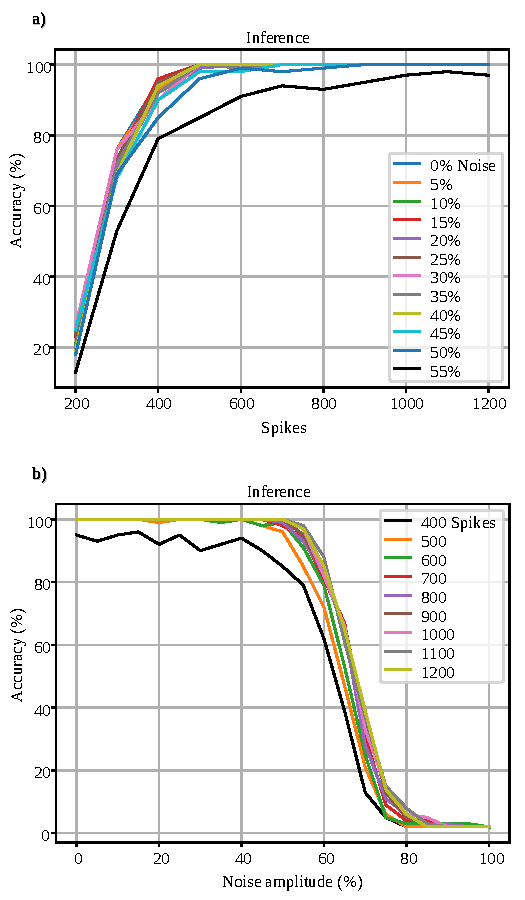
\includegraphics[width=0.5\columnwidth]{./chapters/sbs_accelerator/figures/accuracy_vs_noise_pu_fp.pdf}
	\caption{Noise tolerance on hardware PU with standard floating-point (IEEE 754) computation (benchmark/reference), (a) exhibits accuracy degradation applying $50\%$ of noise amplitude, and (b) illustrates convergence of inference with $400$ spikes.}
	\label{fig:accuracy_vs_noise_pu_fp}
\end{figure*}

\subsection{Design Exploration with Hybrid Custom Floating-Point and Logarithmic Computation}

In this section, it is presented a design exploration to evaluate the proposed approach for \gls{sbs} neural network inference using hybrid custom floating-point and logarithmic approximation. First, the synaptic weight matrix of each layer is examined in order to determine the minimum requirements for numeric representation and memory storage. Second, the proposed dot-product architecture is implemented using the minimal floating-point and logarithmic representation as design parameters. Finally, it is presented an evaluation of the overall performance, inference accuracy, resource utilization, and power dissipation.

\subsubsection{Parameters for Numeric Representation of Synaptic Weight Matrix}
\label{sec:parameters}

	The parameters for numerical representation of the synaptic weight matrices is obtained from their $\log_2$-histograms presented in {\Fig{fig:log2histogram}}. These histograms show the distribution of synaptic weight values in each matrix. The histograms show that the minimum integer exponent value is $-13$. Hence, applying {\Equ{eq:exp_max}} and {\Equ{eq:bits_exp}} to the given \gls{sbs} network, results $E_{\min}=-13$ and $N_E=4$, respectively. Therefore, 4-bits are used for the absolute binary representation of the exponents.


For quality configurability, the mantissa bit-width is a knob parameter that is tuned by the designer. This procedure leverages the builtin error-tolerance of neural networks and performs a trade-off between resource utilization and \gls{qor}. In the following subsection, a case study is presented with 1-bit mantissa. This corresponds to the custom floating-point approximation.

\begin{figure*}[b!]
	\centering
	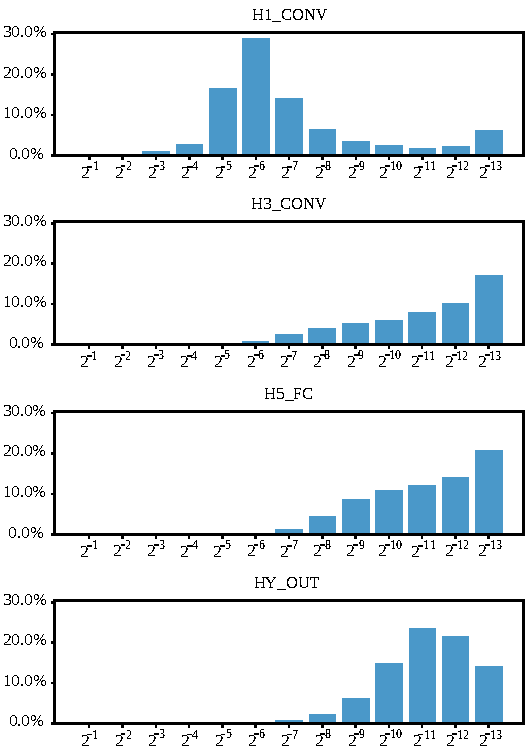
\includegraphics[width=0.5\columnwidth]{./chapters/sbs_accelerator/figures/log2_histogram.pdf}
	\caption{$\log_2$-histogram of each synaptic weight matrix showing the percentage of matrix elements with given integer exponent.}\label{fig:log2histogram}
\end{figure*}

\subsubsection{Design Exploration for Dot-product with Hybrid Custom Floating-Point Computation}
For this design exploration, a custom floating-point representation is composed of 4-bit exponent and 1-bit mantissa. This format is used for the synaptic weight vector on the proposed dot-product architecture. Each \emph{Conv} \gls{pu} instantiates an on-chip stationary weight matrix for $52,000$ entries of 5-bit. The available memory size is large enough to store $W\in\mathbb{R}^{5\times 5\times 2\times 32}$ and $W\in\mathbb{R}^{5\times 5\times 32\times 64}$ for \emph{H1\_CONV} and \emph{H3\_CONV}, respectively. The same dot-product architecture is implemented in the processing unit of the fully connected layer (\emph{FC}). However, due to lack of BRAM resources, this \gls{pu} can not instantiate on-chip stationary synaptic weight matrix. Instead, \emph{FC} receives the $\vec{W}(s_t)$ (weight vectors) during operation as well as $\vec{h}_\mu$ and $S_t$. The hardware mapping and the computation schedule of this implementation are displayed in \Tab{tab:latency_cfp} and \Fig{fig:latency_pu_cfp_cycle}.

As shown in the computation schedule in \Tab{tab:latency_cfp} and \Fig{fig:latency_pu_cfp_cycle}, this implementation presents a maximum hardware \gls{pu} latency of \unit[1.30]{ms} according to \Equ{eq:time_pu}, and \gls{cpu} latency of \unit[1.67]{ms}. Therefore, applying \Equ{eq:time_spike}, the total latency is \unit[1.67]{ms} per spike cycle as shown in \Fig{fig:latency_pu_cfp_cycle}. In this case, the cyclic bottleneck in each \gls{sbs} spike is in the \gls{cpu} performance.

This configuration achieves an accuracy of $98.97\%$ correct classification on the $10,000$ image test set with $1000$ spikes. This indicates an accuracy degradation of $0.33\%$. To monitoring output quality, the noise tolerance plot in \Fig{fig:accuracy_vs_noise_pu_cfp} revels accuracy degradation for noise higher than $50\%$ on the input images, and convergence of inference with $400$ spikes. Thus, the particular \gls{sbs} network implementation under approximate processing effects demonstrates a minimal impact on the overall accuracy. This reveals an inherent error resilience, and hence, remaining approximation budget.

The post-implementation resource utilization and power dissipation of this design are shown in \Tab{tab:resource_cfp}.

\begin{table}[h!]\centering
	\caption{Resource utilization and power dissipation of processing units with hybrid custom floating-point approximation.}\label{tab:resource_cfp}
	\scriptsize
	\begin{tabular}{lrrrrrrr}\toprule
		\textbf{PU} & &\textbf{LUT} &\textbf{FF} &\textbf{DSP} &\textbf{BRAM 18K} &\textbf{Power (mW)} \\\midrule
		Conv & &3,139 &4,850 &19 &25 &82 \\
		FC & &3,265 &5,188 &8 &9 &66 \\
		\bottomrule
	\end{tabular}
\end{table}


\begin{table}[t!]\centering
	\caption{Performance of hardware processing units with hybrid custom floating-point approximation.}\label{tab:latency_cfp}
	\scriptsize
	\begin{tabular}{llrrrrrr}\toprule
		\multicolumn{2}{c}{\textbf{Hardware mapping}} & &\multicolumn{4}{c}{\textbf{Computation schedule (ms)}} \\\cmidrule{1-2}\cmidrule{4-7}
		\textbf{Layer} &\textbf{PU} & &$t_s$ &$t_{CPU}$ &$t_{PU}$ &$t_f$ \\\midrule
		HX\_IN &Spike & &0 &0.055 &0.307 &0.362 \\
		H1\_CONV &Conv1 & &0.057 &0.654 &1.309 &2.020 \\
		\multirow{2}{*}{H2\_POOL} &Pool1 & &0.713 &0.131 &1.098 &1.942 \\
		&Pool2 & &0.845 &0.125 &1.098 &2.068 \\
		\multirow{2}{*}{H3\_CONV} &Conv2 & &0.972 &0.285 &1.199 &2.456 \\
		&Conv3 & &1.258 &0.279 &1.184 &2.721 \\
		H4\_POOL &Pool3 & &1.538 &0.037 &0.484 &2.059 \\
		H5\_FC &FC & &1.577 &0.091 &0.438 &2.106 \\
		HY\_OUT &CPU & &1.669 &0.004 &0 &1.673 \\
		\bottomrule
	\end{tabular}
\end{table}

\begin{figure*}[b!]
	\centering
	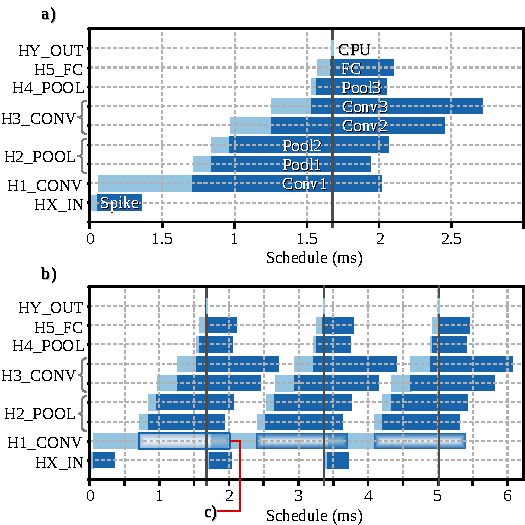
\includegraphics[width=0.5\columnwidth]{./chapters/sbs_accelerator/figures/latency_cfp_cycle.pdf}
	\caption{Performance on processing units with hybrid custom floating-point approximation, (a) exhibits computation schedule, (b) presents cyclic computation schedule, and (c) shows the performance of \emph{Conv2} from a previous computation cycle during the preprocessing of \emph{H1\_CONV} on the current computation cycle without bottleneck.}
	\label{fig:latency_pu_cfp_cycle}
\end{figure*}

\begin{figure*}[b!]
	\centering
	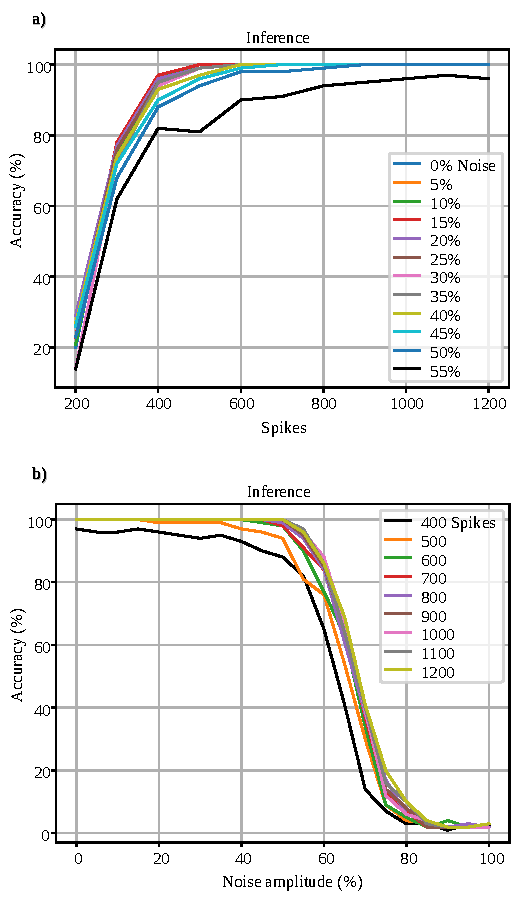
\includegraphics[width=0.5\columnwidth]{./chapters/sbs_accelerator/figures/accuracy_vs_noise_pu_cfp(4-bit-exponent_1-bit-mantissa).pdf}
	\caption{Noise tolerance on hardware PU with custom floating-point approximation, (a) exhibits accuracy degradation applying $50\%$ of noise amplitude, and (b) illustrates convergence of inference with $400$ spikes.}
	\label{fig:accuracy_vs_noise_pu_cfp}
\end{figure*}

\subsubsection{Design Exploration for Dot-Product whit Hybrid Logarithmic Computation}
For this design, 4-bit integer exponent are used for logarithmic representation of the synaptic weight matrix. Each \emph{Conv} processing unit implements the proposed dot-product architecture including an on-chip stationary weight matrix for $52,000$ entries of 4-bit integer each one to store $W\in\mathbb{N}^{5\times 5\times 2\times 32}$ and $W\in\mathbb{N}^{5\times 5\times 32\times 64}$ for \emph{H1\_CONV} and \emph{H3\_CONV}, respectively. The same dot-product architecture is implemented in the \emph{FC} processing unit without stationary synaptic weight matrix. The hardware assignment and the computation schedule of this implementation are displayed in \Tab{tab:latency_log} and \Fig{fig:latency_pu_log_cycle}.

As shown in the computation schedule in \Tab{tab:latency_log} and \Fig{fig:latency_pu_log_cycle}, this implementation presents a maximum hardware \gls{pu} latency of \unit[1.27]{ms} (according to \Equ{eq:time_pu}), and \gls{cpu} latency of \unit[1.67]{ms}. Therefore, applying \Equ{eq:time_spike}, gives \unit[1.67]{ms} as latency per spike cycle as shown in \Fig{fig:latency_pu_log_cycle}. In this case, the cyclic bottleneck is in the \gls{cpu} performance.

This quality configuration achieves an accuracy of $98.84\%$ correct classification on the $10,000$ image test set with $1000$ spikes. This indicates an accuracy degradation of $0.46\%$. To monitor output quality, the noise tolerance plot in \Fig{fig:accuracy_vs_noise_pu_log} revels accuracy degradation having $40\%$ noise on the input images, and convergence of inference with $600$ spikes. The particular \gls{sbs} network implementation under approximate processing demonstrates a minor impact on the overall accuracy. As the most efficient setup and yet the worst-case quality configuration, this exhibits remaining budget for further approximate processing approaches.

The post-implementation resource utilization and power dissipation are shown in \Tab{tab:resource_log}.

\begin{table}[t!]\centering
	\caption{Performance of hardware processing units with hybrid logarithmic approximation.}\label{tab:latency_log}
	\scriptsize
	\begin{tabular}{llrrrrrr}\toprule
		\multicolumn{2}{c}{\textbf{Hardware mapping}} & &\multicolumn{4}{c}{\textbf{Computation schedule (ms)}} \\\cmidrule{1-2}\cmidrule{4-7}
		\textbf{Layer} &\textbf{PU} & &$t_s$ &$t_{CPU}$ &$t_{PU}$ &$t_f$ \\\midrule
		HX\_IN &Spike & &0 &0.055 &0.264 &0.319 \\
		H1\_CONV &Conv1 & &0.057 &0.655 &1.271 &1.983 \\
		\multirow{2}{*}{H2\_POOL} &Pool1 & &0.714 &0.130 &1.074 &1.918 \\
		&Pool2 & &0.845 &0.126 &1.106 &2.077 \\
		\multirow{2}{*}{H3\_CONV} &Conv2 & &0.973 &0.285 &1.179 &2.437 \\
		&Conv3 & &1.258 &0.278 &1.176 &2.712 \\
		H4\_POOL &Pool3 & &1.538 &0.037 &0.488 &2.063 \\
		H5\_FC &FC & &1.577 &0.091 &0.388 &2.056 \\
		HY\_OUT &CPU & &1.669 &0.004 &0 &1.673 \\
		\bottomrule
	\end{tabular}
\end{table}

\begin{figure*}[b!]
	\centering
	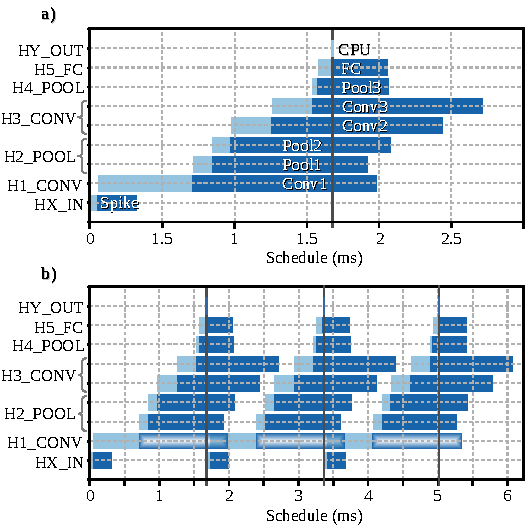
\includegraphics[width=0.5\columnwidth]{./chapters/sbs_accelerator/figures/latency_log_cycle.pdf}
	\caption{Performance of processing units with hybrid logarithmic approximation, (a) exhibits computation schedule, and (b) illustrates cyclic computation schedule.}
	\label{fig:latency_pu_log_cycle}
\end{figure*}

\begin{table}[!h]\centering
	\caption{Resource utilization and power dissipation of processing units with hybrid logarithmic approximation.}\label{tab:resource_log}
	\scriptsize
\begin{tabular}{lrrrrrrr}\toprule
	\textbf{PU} & &\textbf{LUT} &\textbf{FF} &\textbf{DSP} &\textbf{BRAM 18K} &\textbf{Power (mW)} \\\midrule
	Conv & &3,086 &4,804 &19 &21 &78 \\
	FC & &3,046 &4,873 &8 &8 &66 \\
	\bottomrule
\end{tabular}
\end{table}

%\begin{figure}[!h]
%	\centering
%	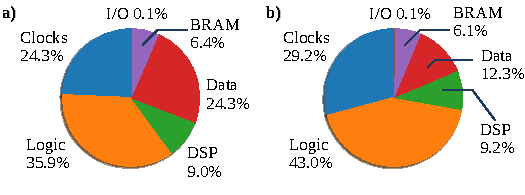
\includegraphics[width=1\columnwidth]{../figures/power_dissipation_breakdown_log-4.pdf}
%	\caption{Power dissipation breakdown of processing units with hybrid logarithmic approximation, (a) \emph{Conv}, and (b) \emph{FC}.}
%	\label{fig:power_dissipation_breakdown_log_4}
%\end{figure}



\begin{figure*}[b!]
	\centering
	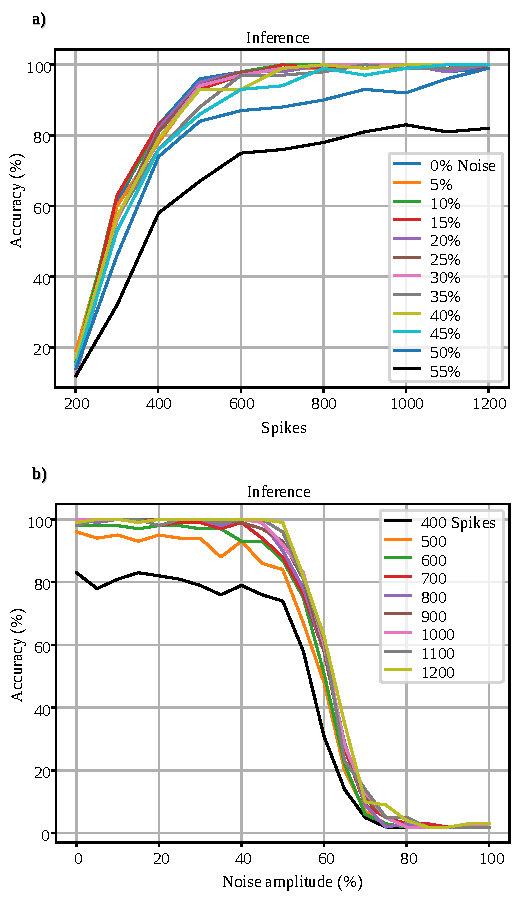
\includegraphics[width=0.5\columnwidth]{./chapters/sbs_accelerator/figures/accuracy_vs_noise_pu_log.pdf}
	\caption{Noise tolerance on hardware PU with hybrid logarithmic approximation, (a) exhibits accuracy degradation applying $40\%$ of noise amplitude, (b) illustrates convergence of inference with $600$ spikes.}
	\label{fig:accuracy_vs_noise_pu_log}
\end{figure*}


\subsection{Results and Discussion}
As benchmark, the \gls{sbs} network inference on embedded \gls{cpu} using standard 32-bit floating-point achieves an accuracy of $99.3\%$ with a latency of $T_{SC} = 34.28 ms$. As a second reference point, the network simulation on hardware processing units with standard floating-point achieves an accuracy of $98.98\%$ with a latency $T_{SC}=3.18 ms$. As result, this design get $10.7\times$ latency enhancement and an accuracy degradation of $0.32\%$. The tolerance plot in \Fig{fig:accuracy_vs_noise_pu_fp} reveals accuracy degradation having $50\%$ noise on the input images, and convergence of inference with $400$ spikes. In this case, the \gls{sbs} network deployment with precise computing proves extraordinary inherent error resilience, and hence, this represents a great potential for approximate processing.

As a demonstration of the proposed dot-product architecture, the \gls{sbs} network inference on hardware \glspl{pu} with synaptic representation using 5-bit custom floating-point (4-bit exponent, 1-bit mantissa) and 4-bit logarithmic (4-bit exponent) achieve $20.5\times$ latency enhancement and accuracy of $98.97\%$ and $98.84\%$, respectively. This results in accuracy degradation of $0.33\%$ and $0.46\%$, respectively. To monitor output quality, the noise tolerance plot in \Fig{fig:accuracy_vs_noise_pu_cfp} and \Fig{fig:accuracy_vs_noise_pu_log} reveal accuracy degradation when having $50\%$ and $40\%$ noise on the input images, and convergence of inference with $400$ and $600$ spikes, respectively. Therefore, the design exploration under the proposed approximate computing approach indicates sufficient inherent error resilience for further or more aggressive approximation approaches.

Regarding resource utilization and power dissipation with the proposed approach, \emph{Conv} processing units have a $43.24\%$ reduction of BRAM, and $12.35\%$ of improvement in energy efficiency over the standard floating-point implementation. However, the proposed approach does not reuse the available floating-point operator cores instantiated from other computational sections (see {\Tab{tab:LogiCORE}}). Therefore, the logic required for the dot-product must be implemented, which is reflected as additional utilization of \gls{lut} and \gls{ff} resources. The experimental results of the design exploration are summarized in \Tab{tab:results}. The platform implementations are summarized in \Tab{tab:platform_comparison}, and their power dissipation breakdowns are presented in \Fig{fig:platform_power_dissipation_breakdown}.

\begin{table*}[!t]
	\begin{threeparttable}
		\centering
		\caption{Experimental results.}\label{tab:results}
		\scriptsize
\begin{tabular}{lrrrrrrrrrrrr}\toprule
	\multirow{2}{*}{\textbf{Dot-product}} &\multirow{2}{*}{\textbf{PU}} &\multicolumn{4}{c}{\textbf{Post-implementation resource utilization}} &\multirow{2}{*}{\textbf{Power (mW)}} &\multicolumn{2}{c}{\textbf{Latency}} & &\multicolumn{2}{c}{\textbf{Accuracy (\%)\tnote{e}}} \\\cmidrule{3-6}\cmidrule{8-9}\cmidrule{11-12}
			& &\textbf{LUT} &\textbf{FF} &\textbf{DSP} &\textbf{BRAM 18K} & &(ms)&\textbf{Gain\tnote{d}} & &\textbf{Noise 0\%} &\textbf{50\%} \\\midrule
				\multirow{2}{*}{Standard \gls{fp}\tnote{a}} &Conv &2,765 &4,366 &19 &37 &89 &\multirow{2}{*}{3.183} &\multirow{2}{*}{10.77x} & &\multirow{2}{*}{98.98} &\multirow{2}{*}{98.63} \\
				&FC &2,649 &4,189 &8 &9 &66 & & & & & \\
				& & & & & & & & & & & \\
				\multirow{2}{*}{Hybrid custom \gls{fp}\tnote{b}} &Conv &3,139 &4,850 &19 &25 &82 &\multirow{2}{*}{1.673} &\multirow{2}{*}{20.49x} & &\multirow{2}{*}{98.97} &\multirow{2}{*}{98.47} \\
				&FC &3,265 &5,188 &8 &9 &66 & & & & & \\
				& & & & & & & & & & & \\
				\multirow{2}{*}{Hybrid log\tnote{c}} &Conv &3,086 &4,804 &19 &21 &78 &\multirow{2}{*}{1.673} &\multirow{2}{*}{20.49x} & &\multirow{2}{*}{98.84} &\multirow{2}{*}{95.22} \\
				&FC &3,046 &4,873 &8 &8 &66 & & & & & \\
				\bottomrule
			\end{tabular}
		\begin{tablenotes}
			\scriptsize
			\item[a] Reference with standard floating-point arithmetic (IEEE 754).
			\item[b] Synaptic weight with number representation composed of 4-bit exponent and 1-bit mantissa.
			\item[c] Synaptic weight with number representation composed of 4-bit exponent.
			\item[d] Acceleration with respect to the computation on embedded CPU (ARM Cortex-A9 at 666 MHz) with latency $T_{SC} = 34.28 ms$.
			\item[e] Accuracy on 10,000 image test set with 1000 spikes.
		\end{tablenotes}
	\end{threeparttable}
\end{table*}


\begin{table*}[!t]
	\begin{threeparttable}
		\centering
		\caption{Platform implementations.}\label{tab:platform_comparison}
		\scriptsize
		\begin{tabular}{lrrrrrrrrrr}\toprule
			\multirow{2}{*}{\textbf{Platform implementation}} &\multicolumn{4}{c}{\textbf{Post-implementation resource utilization}} &\multirow{2}{*}{\textbf{Power (W)}} &\multirow{2}{*}{\textbf{Clk (MHz)}} &\multicolumn{2}{c}{\textbf{Latency}} &\multirow{2}{*}{\textbf{Accu (\%)\tnote{f}}} \\\cmidrule{2-5}\cmidrule{8-9}
			&\textbf{LUT} &\textbf{FF} &\textbf{DSP} &\textbf{BRAM 18K} & & &\textbf{(ms)} &\textbf{Gain\tnote{e}} & \\\midrule
			\cite{nevarez2020accelerator}\tnote{a} &42,740 &57,118 &49 &92 &2.519 &250 &4.65 &7.4x &99.02 \\
			This work (standard \gls{fp})\tnote{b} &39,514 &56,036 &82 &180 &2.420 &200 &3.18 &10.7x &98.98 \\
			This work (hybrid custom \gls{fp})\tnote{c} &42,021 &58,759 &82 &156 &2.369 &200 &1.67 &20.5x &98.97 \\
			This work (hybrid log)\tnote{d} &41,060 &57,862 &82 &148 &2.324 &200 &1.67 &20.5x &98.84 \\
			\bottomrule
		\end{tabular}
		\begin{tablenotes}
			\scriptsize
			\item[a] Reference architecture with homogeneous AUs using standard floating-point arithmetic (IEEE 754).
			\item[b] Reference architecture with specialized heterogeneous PUs using standard floating-point arithmetic (IEEE 754).
			\item[c] Proposed architecture with specialized heterogeneous PUs using synaptic weight with number representation composed of 4-bit exponent and 1-bit mantissa.
			\item[d] Proposed architecture with specialized heterogeneous PUs using synaptic weight with number representation composed of 4-bit exponent.
			\item[e] Acceleration with respect to the computation on embedded CPU (ARM Cortex-A9 at 666 MHz) with latency $T_{SC} = 34.28 ms$.
			\item[f] Accuracy on 10,000 image test set with 1000 spikes.
		\end{tablenotes}
	\end{threeparttable}
\end{table*}

\begin{figure*}[b!]
	\centering
	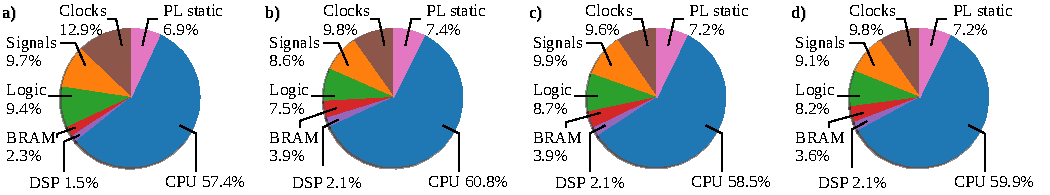
\includegraphics[width=\columnwidth]{./chapters/sbs_accelerator/figures/platform_power_dissipation_breakdown.pdf}
	\caption{Power dissipation breakdown of platform implementations, (a) \cite{nevarez2020accelerator} architecture with homogeneous AUs using standard floating-point arithmetic (IEEE 754), (b) reference architecture with specialized heterogeneous PUs using standard floating-point arithmetic (IEEE 754), (c) proposed architecture with hybrid custom floating-point approximation, and (d) proposed architecture with hybrid logarithmic approximation.}
	\label{fig:platform_power_dissipation_breakdown}
\end{figure*}